\section{Design of Software System}
\label{sec:design}

\subsection{System Overview}

The Introspection AI Assistant represents a comprehensive psychological support system implemented as a WeChat Mini Program, designed to provide accessible, non-clinical emotional support through advanced artificial intelligence technologies. The system integrates multiple specialized AI agents orchestrated through a sophisticated LangGraph-based architecture, enabling real-time emotional analysis, event extraction, and personalized mental health insights.

The system architecture employs a microservices design pattern with clear separation of concerns, facilitating maintainability, scalability, and fault tolerance. Each component operates independently while communicating through well-defined RESTful APIs, ensuring robust system performance under varying operational conditions.

\subsection{System Architecture}

\subsubsection{Core Processing Framework}

The system employs a sophisticated LangGraph-based workflow architecture comprising eight specialized processing nodes, each responsible for distinct aspects of the psychological support pipeline:

\begin{enumerate}
\item \textbf{Input Preprocessing}: Message sanitization, context initialization, and feature extraction
\item \textbf{Crisis Detection}: Real-time identification of high-risk psychological states requiring immediate intervention
\item \textbf{Context Construction}: Integration of user profile, conversation history, and long-term memory systems
\item \textbf{Information Retrieval}: Conditional activation of external knowledge base searches
\item \textbf{Strategic Planning}: Dynamic conversation strategy formulation based on therapeutic objectives
\item \textbf{Guided Inquiry}: Systematic information gathering through structured questioning protocols
\item \textbf{Pattern Analysis}: Behavioral and emotional pattern recognition across conversation sessions
\item \textbf{Response Generation}: Contextually appropriate therapeutic response synthesis
\end{enumerate}

\begin{figure}[h]
\centering
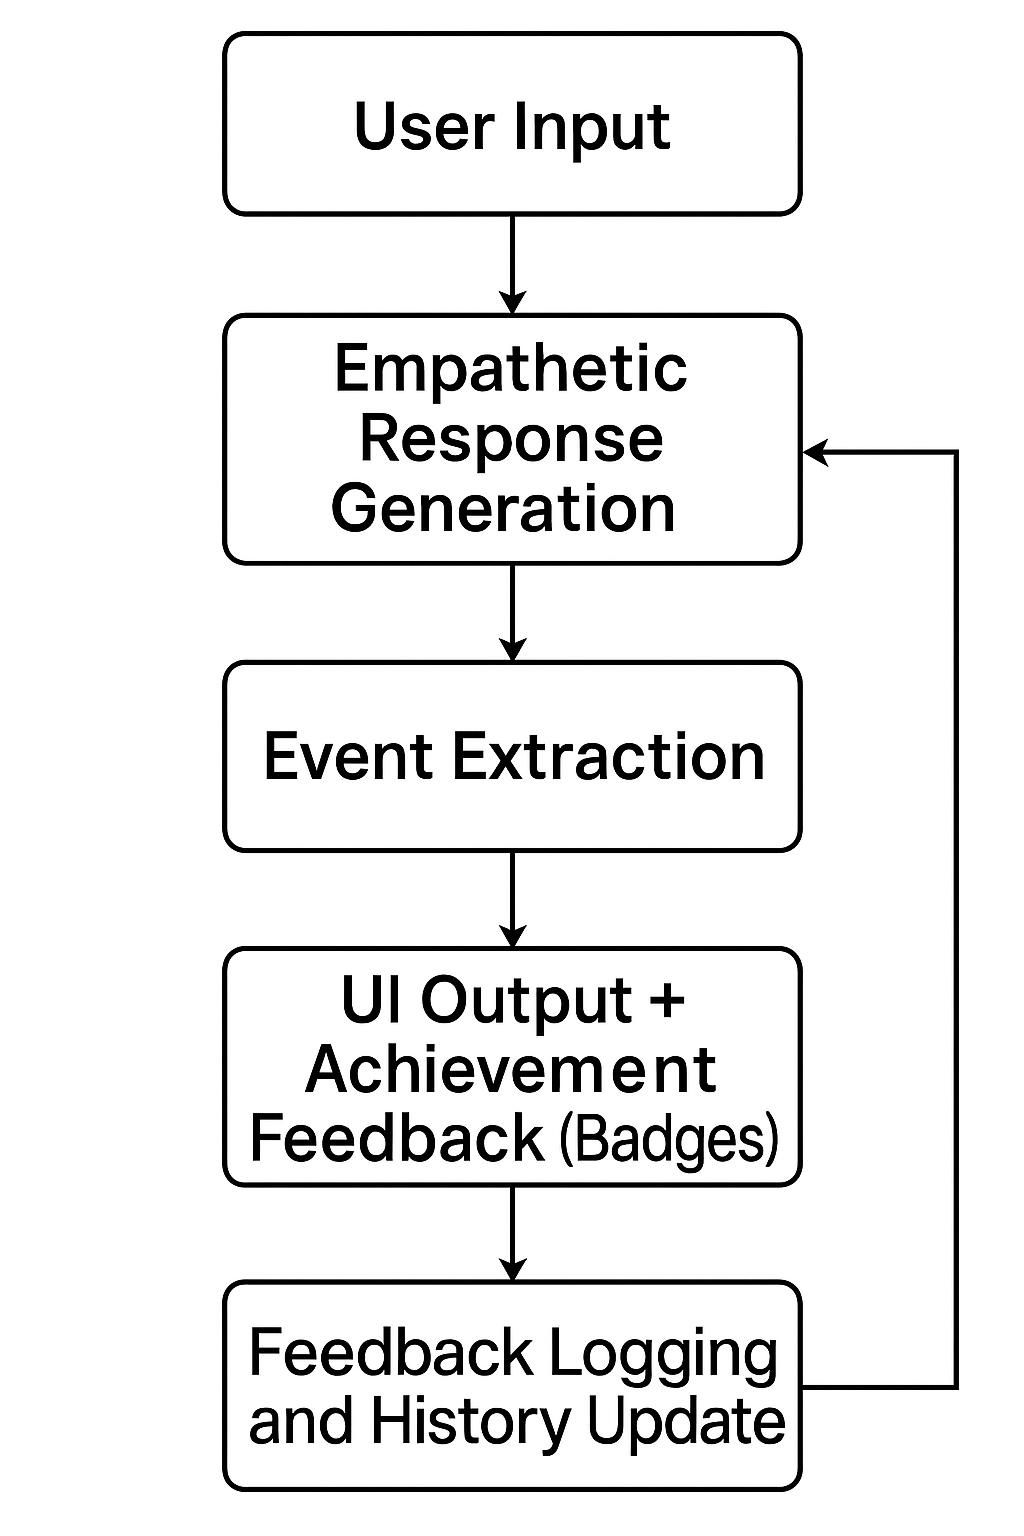
\includegraphics[width=0.8\textwidth]{figs/system_architecture.png}
\caption{LangGraph-based system architecture with parallel processing nodes}
\label{fig:system_architecture}
\end{figure}

\subsubsection{Processing Pipeline Implementation}

The system processes user input through a sophisticated parallel execution model with conditional routing mechanisms:

\begin{verbatim}
[ User Input ] → [ Preprocessing ] → [ Crisis Detection ]
                                    ↓
[ Context Building ] ← [ Information Retrieval ] ← [ Strategic Planning ]
                                    ↓
[ Guided Inquiry ] → [ Pattern Analysis ] → [ Response Generation ]
                                    ↓
[ Event Extraction ] → [ Data Persistence ] → [ User Feedback ]
\end{verbatim}

This architecture enables concurrent processing of non-dependent operations while maintaining strict sequential execution for operations requiring previous results, optimizing both response latency and computational efficiency.

\subsection{User Interface Design}

\subsubsection{Platform Selection and Integration}

The system leverages the WeChat Mini Program ecosystem to maximize user accessibility and adoption rates. This platform choice eliminates software installation barriers while providing familiar interaction paradigms for the target demographic. The interface design adheres to contemporary instant messaging conventions while incorporating specialized features for psychological support.

\begin{figure}[h]
\centering
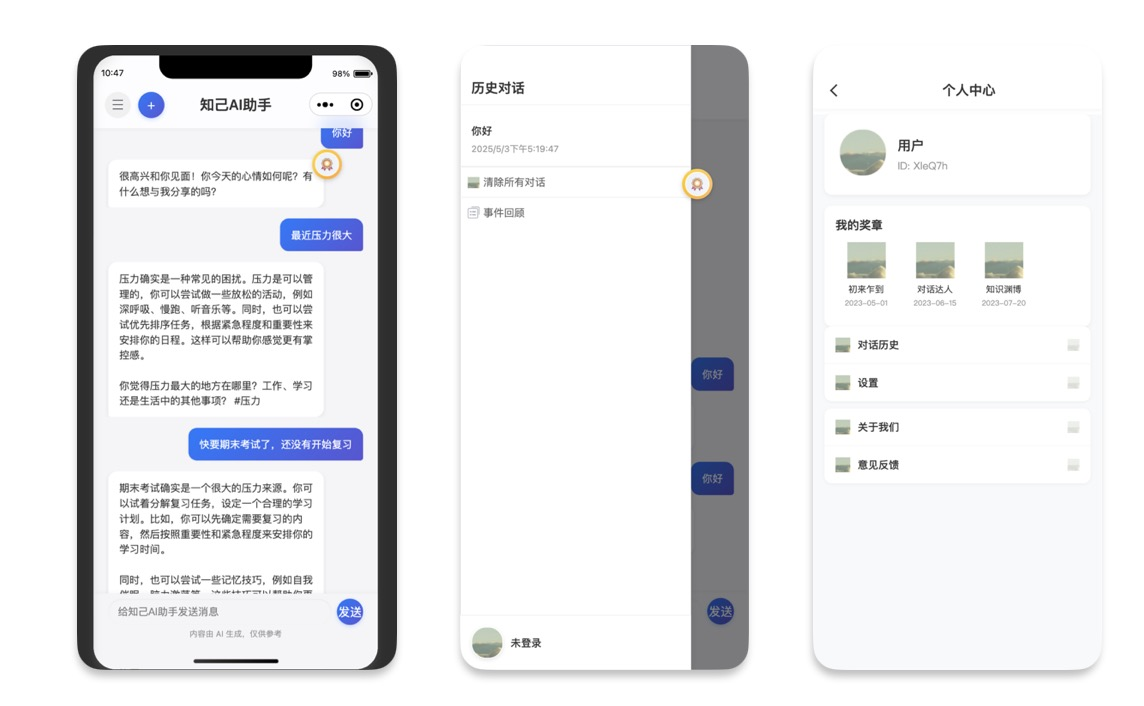
\includegraphics[width=0.6\textwidth]{figs/ui_chat_screen.png}
\caption{Conversational interface with integrated emotional feedback systems}
\label{fig:ui_chat_screen}
\end{figure}

\subsubsection{Interface Components}

The user interface incorporates several specialized components optimized for psychological support applications:

\begin{itemize}
\item \textbf{Conversational Interface}: Primary interaction area featuring message threading and typing indicators
\item \textbf{Emotional State Indicators}: Real-time visualization of detected emotional states and intensity levels
\item \textbf{Navigation Panel}: Access to conversation history, emotional analysis, and achievement tracking
\item \textbf{Event Timeline}: Chronological display of extracted psychological events and milestones
\item \textbf{Achievement System}: Gamified progress tracking through earned badges and recognition tokens
\end{itemize}

\subsection{Functional Module Implementation}

\subsubsection{Core System Components}

The system architecture integrates multiple specialized modules, each addressing specific aspects of psychological support delivery:

\begin{table}[h]
\centering
\begin{tabular}{|l|p{8cm}|}
\hline
\textbf{Module} & \textbf{Implementation Description} \\
\hline
Empathetic Response Generation & Utilizes fine-tuned language models to generate therapeutically appropriate responses with emotional validation \\
\hline
Real-time Emotion Analysis & Employs SnowNLP sentiment analysis combined with LLM-based emotion classification for comprehensive emotional state assessment \\
\hline
Event Extraction System & Asynchronous processing pipeline for identifying and categorizing psychologically significant events from conversation data \\
\hline
Guided Inquiry Framework & Structured questioning protocols designed to systematically gather complete event information \\
\hline
Pattern Recognition Engine & Behavioral pattern analysis across multiple conversation sessions to identify recurring themes and concerns \\
\hline
Crisis Detection System & Real-time monitoring for high-risk indicators with automated escalation protocols \\
\hline
\end{tabular}
\caption{Core functional modules and their implementation characteristics}
\label{tab:functional_modules}
\end{table}

\begin{figure}[h]
\centering
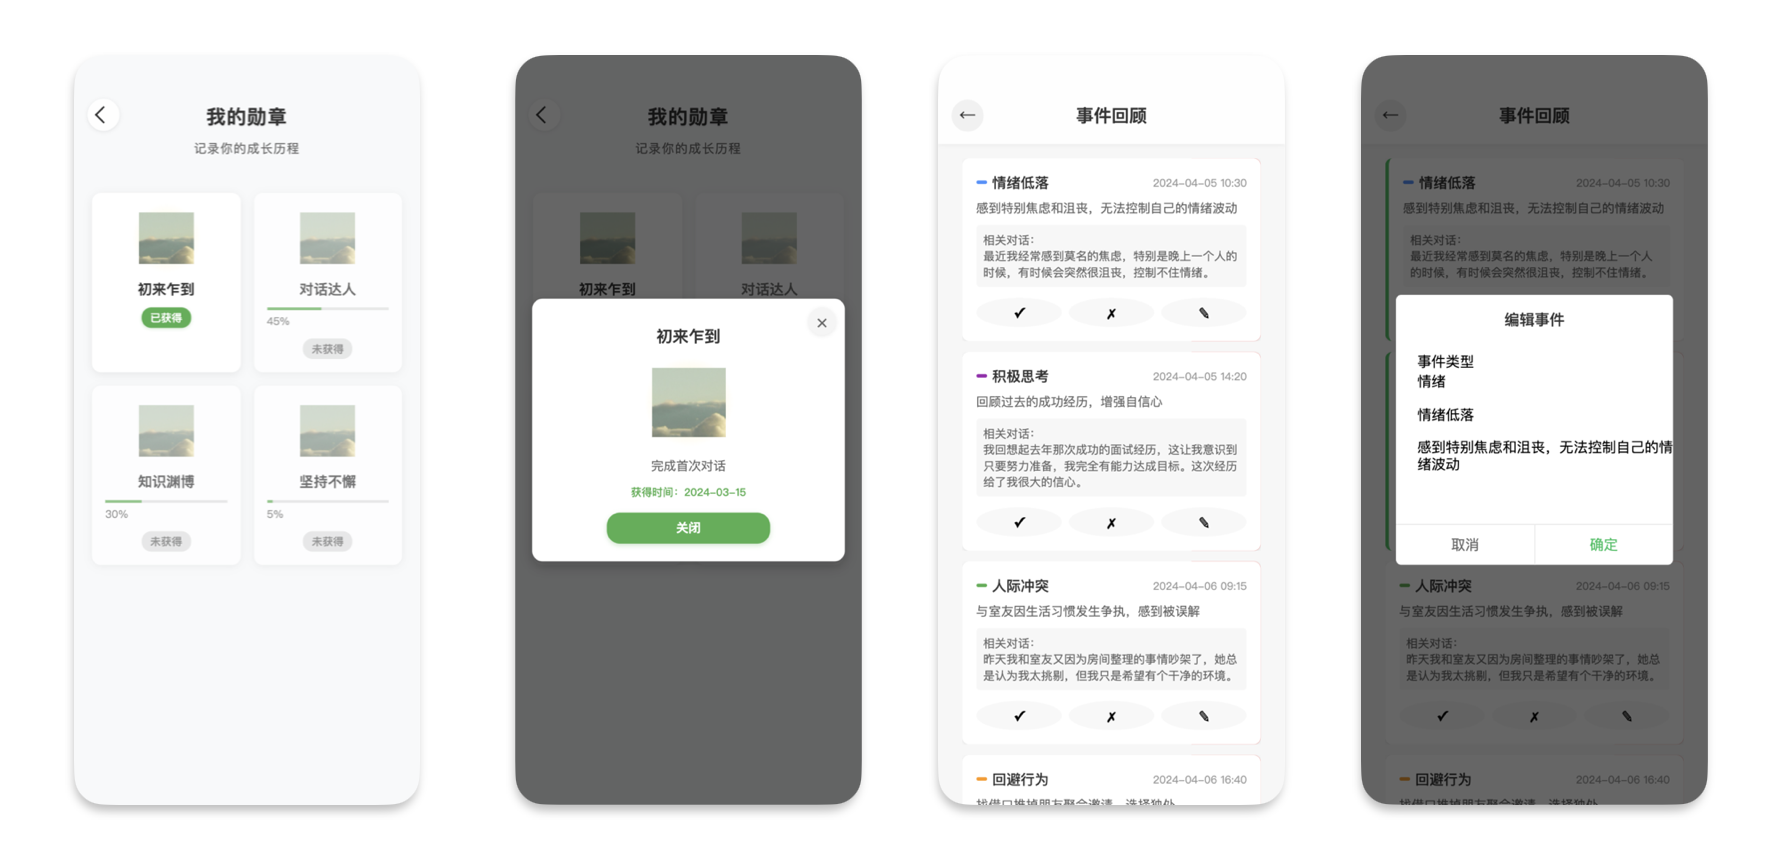
\includegraphics[width=0.8\textwidth]{figs/medal_event_system.png}
\caption{Achievement system and event management interface}
\label{fig:medal_event_system}
\end{figure}

\subsubsection{Advanced Feature Integration}

The system incorporates several advanced features that distinguish it from conventional chatbot implementations:

\begin{itemize}
\item \textbf{Long-term Memory Management}: Persistent storage of conversation context and user psychological profiles with privacy-preserving encryption
\item \textbf{Adaptive Response Strategies}: Dynamic adjustment of therapeutic approaches based on user response patterns and progress indicators
\item \textbf{Comprehensive Analysis Reports}: Automated generation of detailed psychological assessment reports integrating multiple data sources
\item \textbf{Asynchronous Event Processing}: Background extraction and categorization of psychological events to minimize response latency
\end{itemize}

\subsection{Technical Implementation}

\subsubsection{System Architecture Stack}

The technical implementation employs a modern, scalable architecture designed for high availability and performance:

\begin{table}[h]
\centering
\begin{tabular}{|l|l|}
\hline
\textbf{Component} & \textbf{Technology Implementation} \\
\hline
Frontend Platform & WeChat Mini Program (WXML, WXSS, JavaScript) \\
\hline
Backend Framework & Flask-based microservices architecture \\
\hline
Orchestration Engine & LangGraph for AI agent workflow management \\
\hline
Language Models & DeepSeek, Qwen3-32B, OpenAI-compatible APIs \\
\hline
Data Storage & File-based persistence with JSON serialization \\
\hline
\end{tabular}
\caption{Technical implementation stack and architectural components}
\label{tab:technical_stack}
\end{table}

\subsubsection{AI Model Integration}

The system integrates multiple specialized language models to optimize performance across different processing tasks:

\begin{itemize}
\item \textbf{Primary Conversation Model}: DeepSeek-chat model optimized for therapeutic conversation generation with temperature controls for response consistency
\item \textbf{Event Extraction Model}: Qwen3-32B model specialized for structured data extraction from unstructured conversation text
\item \textbf{Emotion Analysis Model}: Hybrid approach combining SnowNLP statistical analysis with LLM-based categorical classification
\item \textbf{Crisis Detection Model}: Fine-tuned classifier for identifying high-risk psychological states with configurable sensitivity thresholds
\end{itemize}

\subsection{Database Design and Data Management}

\subsubsection{Storage Architecture}

The system employs a lightweight, file-based storage architecture optimized for development flexibility and data portability:

\begin{itemize}
\item \textbf{Message Storage}: Session-based JSON files containing conversation history with metadata
\item \textbf{Event Database}: Structured storage of extracted psychological events with temporal indexing
\item \textbf{User Profiles}: Persistent storage of user psychological profiles and preference settings
\item \textbf{Analysis Reports}: Comprehensive psychological assessment reports with export capabilities
\end{itemize}

\subsubsection{Data Flow Management}

The system implements sophisticated data flow management to ensure consistency and performance:

\begin{enumerate}
\item \textbf{Input Validation}: Comprehensive sanitization and validation of user inputs
\item \textbf{Parallel Processing}: Concurrent execution of independent analysis tasks
\item \textbf{Conditional Routing}: Dynamic workflow routing based on processing requirements
\item \textbf{Result Aggregation}: Synthesis of multiple analysis outputs into coherent responses
\item \textbf{Persistent Storage}: Atomic write operations with transactional consistency
\end{enumerate}


\subsection{Performance Optimization}

\subsubsection{System Efficiency Measures}

The system incorporates multiple optimization strategies to ensure responsive performance:

\begin{itemize}
\item \textbf{Asynchronous Processing}: Non-blocking execution of computationally intensive tasks
\item \textbf{Caching Mechanisms}: Strategic caching of frequently accessed data and computed results
\item \textbf{Connection Pooling}: Efficient management of external API connections
\end{itemize}


